\documentclass{article}
\usepackage[T1]{fontenc}
\usepackage{lmodern}
\usepackage{graphicx}
\usepackage{amsmath,amssymb}
\usepackage[a4paper,margin=2cm]{geometry}
\usepackage[absolute,overlay]{textpos}
\setlength{\TPHorizModule}{1mm}
\setlength{\TPVertModule}{1mm}
\usepackage[indonesian]{babel}
\usepackage{hyperref}
\setlength{\emergencystretch}{2em}
% unit: Halaman 75

\begin{document}

% === Halaman 75 (python/native) ===

2. Jika dua huruf terdapat pada kolom kunci yang sama maka tiap huruf 

diganti dengan huruf di bawahnya (bersifat siklik).

Bigram: nq

N

Q

Cipherteks: PX

Bigram: ow

O

W

Cipherteks: WL

75

% deskripsi: gambar native xref 274
\noindent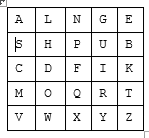
\includegraphics[width=0.85\textwidth]{../../images/python/page_075_img_01.png}

\end{document}
